%\subsection{Superpixel flow}
\label{sec:suppix}

In order to perform the background segments tracking,  we propose a superpixel matching technique, 
which we call superpixel flow. The objective of the superpixel flow is to find the best match for every superpixel $p$ in the first 
frame with one ($p'$) in the next frame, while holding a global flow-like behaviour.

Thus, the superpixelization should maintain certain size homogeneity within a single frame. Some super
pixel techniques can cope with this requirement \cite{c9}\cite{c10}. For the experiments presented 
in this work, we prefer the SLIC method \cite{c9}, which gives
good results in terms of size homogeneity and compactness of the superpixelization. 

%\subsection{Energy Formulation}

Inspired by a large number of optical flow and stereo techniques \cite{c7}\cite{c12}\cite{c13}, 
the superpixel flow is modelled with a pairwise Markov Random Field. The matching is performed via maximum-a-posteriori (MAP) inference on the labeling $l$, which is equivalent to the minimization of an energy function of the form:

\begin{equation}
E(l) = \displaystyle \sum_{p \in \Gamma} D_p(l_p;I_0,I_1) +
\sum_{(p,q): q \in \mathcal{N}_r} S_{p,q}(l_p,l_q) .
\label{eq_energy}
\end{equation}

With $l$ the set of labels of the superpixels in $I_0$,
that match with those in $I_1$, in the super pixel space $\Gamma$. $\mathcal{N}_r$ is a neighbourhood of radius $r$ of the superpixel $p$.
The terms $D$, and $S$ in (\ref{eq_energy}) stand for data term and spatial smoothness term. 
The first one determines how accurate is the labeling in terms
of consistency with the measured data (color, shape,etc.). In the classical optical flow equivalent of this equation,
the data term corresponds to the pixel brightness conservation\cite{c7}\cite{c5}. However, as superpixels are a set
of similar (or somehow homogeneous) pixels, an adequate appearance based feature is a low dimensional
color histogram (with N bins). So, here, $D$ is the Hellinger distance between the histograms:

\begin{equation}
D_p(l_p;I_0,I_1) = \sqrt{ 1 - \frac{1}{\sqrt{\bar{ \boldsymbol{h} }(p) \bar{ \boldsymbol{h} }(p')N^2} } \sum_{i}\sqrt{ \boldsymbol{h}_{i}(p) \boldsymbol{h}_{i}(p')} }.
\label{eq_Dp}
\end{equation}
Where $\textbf{h}(p)$ and $\textbf{h}(p')$ are the color histograms of the superpixel $p$ and its correspondent superpixel in the
second frame $I_1$. For the experiments we used {\it RGB} color histogram with N=3 bins per color.
Note that the low dimensional histogram gives certain robustness against noise,
and slowly changing colors between frames. 

On the other hand, the spatial term is a penalty function for spatial diference of the displacement vectors between neighboring superpixels, where a displacement vector has origin 
in the centroid of the superpixel of the first frame and
end in the centroid of the superpixel of the second frame.

\begin{equation}
S_{p,q}(l_p, l_q) = \lambda(p)
  \sqrt{\frac{|u_{p_c}-u_{q_c}|}{\|p_c-q_c\|}+ \frac{|v_{p_c}-v_{q_c}|}{\|p_c-q_c\|}},
\label{eq_Spq}
\end{equation}
 where, $ \lambda(p) = (1 + \rho(\boldsymbol{h}(p),\boldsymbol{h}(q)))^2 $.

The operator $\rho$ is the Hellinger distance as used in the
data term (\ref{eq_Dp}). The histogram distance is nonetheless computed between adjacent superpixels $p$ and $q$, 
which belong to the first image. The superpixels centroids are noted as $q_c$ and $p_c$, 
and $u_{*}$ and $v_{*}$ are the horizontal and vertical changes between centroids.
This term has a smoothing effect in superpixels that belong to the
same object. It has to be observed that when two close superpixels are different, thus, more probable to
belong to different objects within the image, the term $\lambda$ allows them to have
matches that do not hold the smoothness prior with the same strength. 

%\subsection{Energy Minimization}
\ifcsdef{r@accv_format}{
   \begin{figure}[thpb]
      \centering
      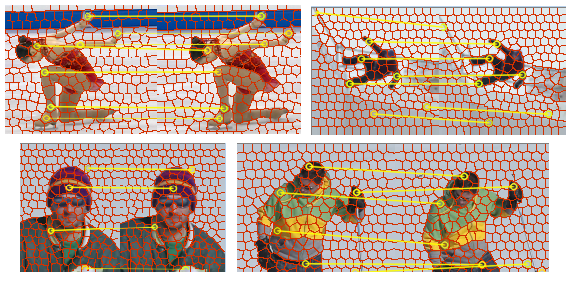
\includegraphics[width=0.935\textwidth]{../images/all_matches.png}
      \caption{The yellow lines show selected superpixel
		matching between pairs of images in several datasets.}
      \label{figurelabel_matchessnow}
   \end{figure}   
	\setlength{\belowcaptionskip}{-10pt}
}{
   \begin{figure}[thpb]
      \centering
      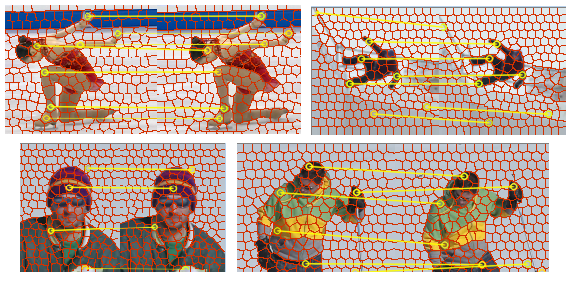
\includegraphics[width=0.5\textwidth]{../images/all_matches.png}
      \caption{The yellow lines show selected superpixel
		matching between pairs of images in several datasets.}
      \label{figurelabel_matchessnow}
   \end{figure}   
	\setlength{\belowcaptionskip}{-10pt}
}

The Quadratic Pseudo-Boolean Optimization (QPBO) \cite{c3}\cite{c4} is used to minimize the proposed energy function, 
by merging a set of candidate matches for every superpixel in the first frame. The candidate matches are generated by assuming 
a proximity prior. This means, every possible match should be inside a seach radius in the second frame. Fig. \ref{figurelabel_matchessnow} shows matching results for several datasets. Observe that the matches are correct even in difficult cases (bottom right).
